%\begin{tikzpicture}
%\begin{axis}[
%    title={SNR-værdier af scaleret billede},
%    xlabel={},
%    ylabel={SNRværdi},
%    width = 0.83*\textwidth,
%    height = 0.5*\textwidth,
%    xtick = {0,1,2,3,4},
%    xmin=0, xmax=4,
%    ymin=0, ymax=8,
%    %x tick label style = {anchor = east},
%    xticklabels={Q10/PC25(12),Q25/PC50(25),Q50/PC75(38),Q75/PC100(50),Q90/PC150(75)},
%    ytick={},
%    legend pos=south east,
%    legend style={
%                at={(1.23,0)}},
%    ymajorgrids=true,
%    grid style=dashed,
%]
% 
%\addplot[
%    color=blue,
%    dashed,
%    ]
%    coordinates {
%    (0,17.02)(1,35.60)(2,35.61)(3,109.19)(4,273.85)
%    };
%\addplot[
%    color=red,
%    dashed,
%    ]
%    coordinates {
%    (0,29.77)(1,66.51)(2,106.58)(3,161.64)(4,292.41)
%    };
%\addplot[
%    color=blue,
%    ]
%    coordinates {
%    (0,10.99)(1,20.44)(2,34.01)(3,53.05)(4,126.98)
%    };
%\addplot[
%    color=red,
%    ]
%    coordinates {
%    (0,23.68)(1,53.04)(2,95.39)(3,155.38)(346.31)
%    };
%]
%\legend{DCT 256x256,DCT 512x512, PCA 256x256, PCA512x512}
%\end {axis}
%\end{tikzpicture}

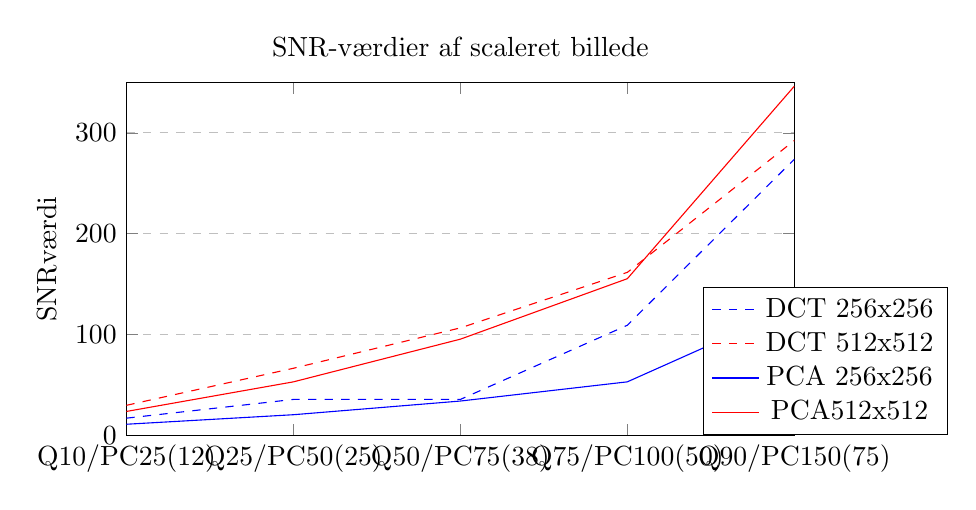
\begin{tikzpicture}
\begin{axis}[
    title={SNR-værdier af scaleret billede},
    xlabel={},
    ylabel={SNRværdi},
    width = 0.83*\textwidth,
    height = 0.5*\textwidth,
    xtick = {0,1,2,3,4},
    xmin=0, xmax=4,
    ymin=0, ymax=350,
    %x tick label style = {anchor = east},
    xticklabels={Q10/PC25(12),Q25/PC50(25),Q50/PC75(38),Q75/PC100(50),Q90/PC150(75)},
    ytick={},
    legend pos=south east,
    legend style={
                at={(1.23,0)}},
    ymajorgrids=true,
    grid style=dashed,
]
 
\addplot[
    color=blue,
    dashed,
    ]
    coordinates {
    (0,17.02)(1,35.60)(2,35.61)(3,109.19)(4,273.85)
    };
\addplot[
    color=red,
    dashed,
    ]
    coordinates {
    (0,29.77)(1,66.51)(2,106.58)(3,161.64)(4,292.41)
    };
\addplot[
    color=blue,
    ]
    coordinates {
    (0,10.99)(1,20.44)(2,34.01)(3,53.05)(4,126.98)
    };
\addplot[
    color=red,
    ]
    coordinates {
    (0,23.68)(1,53.04)(2,95.39)(3,155.38)(4,346.31)
    };
]
\legend{DCT 256x256,DCT 512x512, PCA 256x256, PCA512x512}
\end{axis}
\end{tikzpicture}


%\definecolor{dblue}{HTML}{0000CC}
%\definecolor{lblue}{HTML}{6666FF}
%\definecolor{dgreen}{HTML}{006600}
%\definecolor{lgreen}{HTML}{329932}
%\definecolor{dred}{HTML}{CC0000}
%\definecolor{lred}{HTML}{FF6666}
%\definecolor{dturquoise}{HTML}{2C9C91}
%\definecolor{lturquoise}{HTML}{79E9DE}
%\definecolor{dpurple}{HTML}{660066}
%\definecolor{lpurple}{HTML}{A64CA6}
%\definecolor{dorange}{HTML}{CC8400}
%\definecolor{lorange}{HTML}{FFB732}
%
%\begin{tikzpicture}
%    \begin{axis}[
%        width  = 0.85*\textwidth,
%        height = 8cm,
%        major x tick style = transparent,
%        ymajorgrids = true,
%        xmajorgrids=true,
%    		grid style=dashed,
%        ylabel = {Procent (\%)},
%		xlabel = {Principal Komponenter},
%        ymin=0,
%%		tick style={line width=5pt}
%        legend cell align=left,
%        legend style={
%                at={(0.12,-0.15)},
%                anchor=north west,
%                legend columns= -1,
%                /tikz/every even column/.append style= {column sep=1.0cm}}
%    ]
%        \addplot [ultra thick, dblue] table [col sep=comma, mark = none] {Formalia/Data/T1Q.xlsx};
%        \addplot [ultra thick, lblue] table [col sep=comma, mark = none] {Formalia/Data/T1PCA.xlsx};
%		\addplot [ultra thick, dgreen] table [col sep=comma, mark = none] {Formalia/Data/T2Q.xlsx};
%		\addplot [ultra thick, lgreen] table [col sep=comma, mark = none] {Formalia/Data/T2PCA.xlsx};
%		\addplot [ultra thick, dred] table [col sep=comma, mark = none] {Formalia/Data/T3Q.xlsx};
%		\addplot [ultra thick, lred] table [col sep=comma, mark = none] {Formalia/Data/T3PCA.xlsx};
%		\addplot [ultra thick, dturquoise] table [col sep=comma, mark = none] {Formalia/Data/T4Q.xlsx};
%		\addplot [ultra thick, lturquoise] table [col sep=comma, mark = none] {Formalia/Data/T4PCA.xlsx};
%		\addplot [ultra thick, dpurple] table [col sep=comma, mark = none] {Formalia/Data/T5Q.xlsx};
%		\addplot [ultra thick, lpurple] table [col sep=comma, mark = none] {Formalia/Data/T5PCA.xlsx};
%		\addplot [ultra thick, dorange] table [col sep=comma, mark = none] {Formalia/Data/T6Q.xlsx};
%		\addplot [ultra thick, lorange] table [col sep=comma, mark = none] {Formalia/Data/T6PCA.xlsx};
%%        \legend{Rød, Grøn, Blå , Samlet}
%    \end{axis}
%\label{fig:PCAdiagram}
%\end{tikzpicture}
